\iffalse

INSTRUCTIONS: (if this is not lecture1.tex, use the right file name)

  Clip out the ********* INSERT HERE ********* bits below and insert
appropriate TeX code.  Once you are done with your file, run

  ``latex lecture1.tex''

from a UNIX prompt.  If your LaTeX code is clean, the latex will exit
back to a prompt.  Once this is done, run

  ``dvips lecture1.dvi''

which should print your file to the nearest printer.  There will be
residual files called lecture1.log, lecture1.aux, and lecture1.dvi.
All these can be deleted, but do not delete lecture1.tex.
\fi
%
\documentclass[11pt]{article}
\usepackage{amsfonts}
\usepackage{amsmath}
\usepackage{latexsym}
\usepackage{hyperref}
\usepackage{enumitem}
\usepackage{pdfpages}
\usepackage{graphicx}
\graphicspath{ {./images/} }
\setlength{\oddsidemargin}{.25in}
\setlength{\evensidemargin}{.25in}
\setlength{\textwidth}{6in}
\setlength{\topmargin}{-0.4in}
\setlength{\textheight}{8.5in}

\newcommand{\handout}[5]{
   %\renewcommand{\thepage}{#1-\arabic{page}}
   \noindent
   \begin{center}
   \framebox{
      \vbox{
    \hbox to 5.78in { {\bf Data Structures and Algorithms} \hfill #2 }
       \vspace{4mm}
       \hbox to 5.78in { {\Large \hfill #5  \hfill} }
       \vspace{2mm}
       \hbox to 5.78in { {\it #3 \hfill #4} }
      }
   }
   \end{center}
   \vspace*{4mm}
}

\newcommand{\lecture}[3]{\handout{L#1}{#2}{}{}{#1}}

\def\squarebox#1{\hbox to #1{\hfill\vbox to #1{\vfill}}}
\def\qed{\hspace*{\fill}
        \vbox{\hrule\hbox{\vrule\squarebox{.667em}\vrule}\hrule}}
\newenvironment{solution}{\begin{trivlist}\item[]{\bf Solution:}}
                      {\qed \end{trivlist}}
\newenvironment{solsketch}{\begin{trivlist}\item[]{\bf Solution Sketch:}}
                      {\qed \end{trivlist}}
\newenvironment{proof}{\begin{trivlist}\item[]{\bf Proof:}}
                      {\qed \end{trivlist}}

\newtheorem{theorem}{Theorem}
\newtheorem{corollary}[theorem]{Corollary}
\newtheorem{lemma}[theorem]{Lemma}
\newtheorem{observation}[theorem]{Observation}
\newtheorem{remark}[theorem]{Remark}
\newtheorem{proposition}[theorem]{Proposition}
\newtheorem{definition}[theorem]{Definition}
\newtheorem{Assertion}[theorem]{Assertion}
\newtheorem{fact}[theorem]{Fact}
\newtheorem{hypothesis}[theorem]{Hypothesis}
%\newtheorem{observation}[theorem]{Observation}
%\newtheorem{proposition}[theorem]{Proposition}
\newtheorem{claim}[theorem]{Claim}
\newtheorem{assumption}[theorem]{Assumption}

%Put more macros here, as needed.
\newcommand{\al}{\alpha}
\newcommand{\Z}{\mathbb Z}
\newcommand{\jac}[2]{\left(\frac{#1}{#2}\right)}
\newcommand{\set}[1]{\{#1\}}

\def\ppt{{\sf PPT}}
\def\poly{{\sf poly}}
\def\negl{{\sf negl}}
\def\owf{{\sf OWF}}
\def\owp{{\sf OWP}}
\def\tdp{{\sf TDP}}
\def\prg{{\sf PRG}}
\def\prf{{\sf PRF}}

%end of macros

\title{COSC 336 Assignment 2}
\author{Carmen Phaison and Shannon Ioffe}
\date{February 22, 2023}

\begin{document}

\fbox{
\vbox{
\begin{flushleft}
Shannon Ioffe, Carmen Phaison \\  % authors' names
COSC 237 \\  %class
2/22/2023\\  % date
\end{flushleft}
\center{\Large{\textbf{Assignment 2}}}
%\end{mdframed}
} % end vbox
} % end fbox
\vline

\textbf{Instructions.}
\begin{enumerate}
\item Submit by the date and time indicated on Blackboard. 

\item This is a team assignment. Work in teams of 2-3 students.  Submit on Blackboard one assignment per team, with the names of all students making the team.


\item  For editing your homework. I recommend that you use Latex and Overleaf, see the template files posted on the Blackboard: assignment-template.tex and assignment-template.pdf.
	   
	   \item If a problem has more questions, write down your answers in the same order as the order of questions. In principle, this should help you.

\end{enumerate}
\bigskip

\textbf{Exercise 1.}
\begin{enumerate}[label=\alph*]
\item   Find a $\Theta$ evaluation for the function $(4n + 1) 8^{\log(n^2)}$. (Hint:  $8^{\log(n^2)}$ can be written in a simpler way.)

\medskip Step 1: $(4n + 1) = n$

\medskip Step 2: $8^{\log(n^2)} = (2^3)^{2\log(n)} = 2^{6\log(n)} = 2^{\log(n^6)} = n^6$

\medskip Step 3: $n * n^6 = n^7$

\medskip\textcolor{red}{ {$(4n + 1) 8^{\log(n^2)} = \Theta(n^7)$} }


\item  Give an example of two functions $t_1(n)$ and $t_2(n)$ that satisfy the relations:   $t_1(n) = \Theta(n^2)$, $t_2(n) = \Theta(n^2)$ and $t_1(n) - t_2(n) = o(n^2)$.

\bigskip $t_1(n) = 3n^2 + n$

$t_2(n) = 3n^2$

$(3n^2 + n) - (3n^2) = n$

\textcolor{red}{$n = o(n^2)$}

\item  Give an example of a function $t_1(n)$ such that $t_1(n) = \Theta(t_1(2n))$.

\medskip $t_1(n) = \log(n)$

$t_1(2n) = \log(2n) = \log(n)$

\smallskip\textcolor{red}{$\log(n) = \Theta(\log(2n))$} 

\item   Give an example of a function $t_2(n)$ such that $t_2(n) = o(t_2(2n))$.

$t_2(n) = n!$

$t_2(2n) = 2n!$ 

\textcolor{red}{\smallskip $n! = o(2n!)$}
 
\end{enumerate}

(Note: For (b), (c), (d), seek your examples among polynomials, logarithms, exponentials, factorial.)
\bigskip

\textbf{Exercise 2.}   Fill the table   from Exercise 3-2, page  61 (3-rd edition)  in the textbook (also attached below), except row c, as asked in the exercise.  For example the entry on the first cell in the top row is ``yes" because $\log^k n = O(n^\epsilon)$.  (Note: in row $c$ all the entries are ``no", because $n^{\sin n}$ oscillates.)
\bigskip

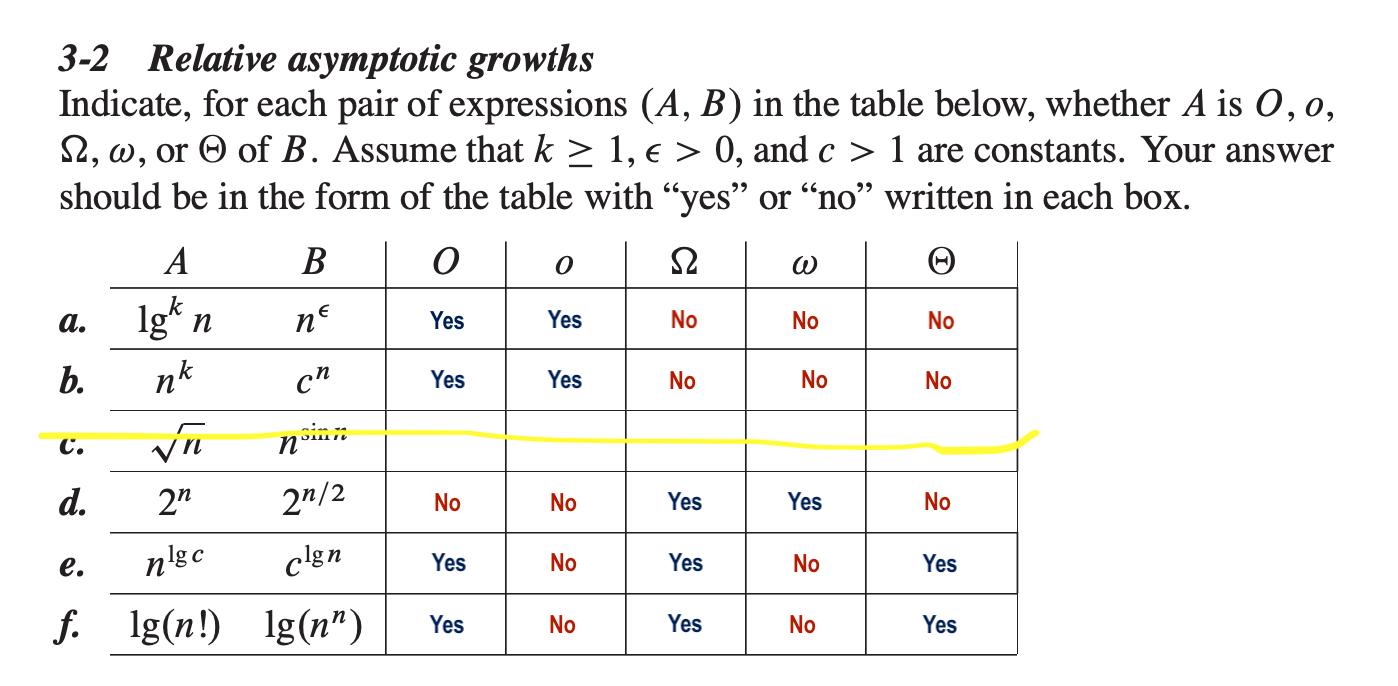
\includegraphics[scale=0.65]{table.png}

\textbf{Exercise 3.}
For each of the following program fragments give a $\Theta(\cdot)$  estimation of the running time as a function of $n$.
\begin{itemize}
\item[(a)]
\begin{verbatim}
sum = 0;
for (int i = 0; i< n * n; i++) {
      for(int j =0;  j < n/2; j++)
    	   sum++;
}

\end{verbatim}

$i(n) = n^2 * j(n)$

$j(n) = n/2$

$i(n) = n^2 * n/2$

\textcolor{red}{= $\Theta(n^3)$}

\medskip\item[(b)]
\begin{verbatim}
 sum = 0;
 for (int i = 0; i< n; i++) {
sum++;}

for(int j = 0;  j < n/2; j++){
      sum++;}

\end{verbatim}

$i(n) = n + j(n)$

$j(n) = n$

$i(n) = 2n$

\textcolor{red}{= $\Theta(n)$}

\medskip\item[(c)]
\begin{verbatim}
 sum = 0;
 for (int i = 0; i< n * n; i++) {
      for(int j = 0;  j < n * n; j++)
           sum++
}
\end{verbatim}

$i(n) = n^2 * j(n)$

$j(n) = n^2$

$i(n) = n^2 * n^2$

\textcolor{red}{= $\Theta(n^4)$}

\medskip\item[(d)]
\begin{verbatim}
 sum = 0;
 for (int i = 1; i< n; i = 2*i)
           sum++

\end{verbatim}

\textcolor{red}{= $\Theta(2^n)$}

\medskip\item[(e)]
\begin{verbatim}
 sum = 0;
 for (int i = 0; i< n; i++) {
      for(int j = 1;  j < n * n; j = 2*j)
           sum++
}
\end{verbatim}

\textcolor{red}{= $\Theta(2^2^n)$}
\end{itemize}
\bigskip
\bigskip
\bigskip
\bigskip
\bigskip
\bigskip
\bigskip
\bigskip
\bigskip
\bigskip
\bigskip
\bigskip
\bigskip
\bigskip
\bigskip
\bigskip
\bigskip
\bigskip



\textbf{Exercise 4.}

(a) Compute the sum $S_1 = 500 + 501+ 502 + 503 + \ldots + 999$ (the sum of all integers from $500$ to $999$). Do not use a program.
\medskip

$n(n+1)/2 = 999(1000)/2 = 499,500$

$n(n+1)/2 = 499(500)/2 = 124,750$

$499,500 - 124,750 = 374,750$
\medskip

\textcolor{red}{374,750}
\bigskip

(b) Compute the sum $S_2 = 1 + 3 + 5 + \ldots + 999$  (the sum of all odd integers from $1$ to $999$).   Do not use a program.
\medskip

$na + d(n-1)/2 = n(1) + 2(n-1)/2 = n+2n-2/2$

$n+2n-2/2 = 500+2(500)-2/2 = 124,998$

\medskip

\textcolor{red}{124,998}
\bigskip

(c) A group of $30$ persons need to form a committee of $3$ persons. How many such committees are possible?
\medskip

\smallskip

$\binom{30}{3} = 30 * 29 * 28/1 * 2 * 3$
\smallskip

$30 * 29 * 28/1 * 2 * 3 = 24360/6 = 4,060$
\medskip

\textcolor{red}{4,060}
\bigskip

(d) Let $C_n$ be the number of committees of $4$ persons selected from a group of $n$ persons.  Is the estimation
$C_n = o(n^3)$ correct? Justify your answer. (Hint: use the formula that gives the number of committees as a function of $n$.)
\medskip

$\binom{n}{4} = n(n-1)(n-2)(n-3)/1 * 2 * 3 * 4$
\medskip

\textcolor{red}{No}
C_n = $\Theta(n^4)$ so, $C_n > (n^3)$ and the estimation should be $\omega(n^3)$ instead.
\bigskip
\bigskip

\textbf{Exercise 5.}
Find a $\Theta(\cdot)$ evaluation for the sum
\[
S = 1\sqrt{1} + 2 \sqrt{2} + \ldots + n \sqrt{n}.
\]
In other words, find a function $f$ such that $S = \Theta(f(n))$.
\medskip

Show the work for both the upper bound and the lower bound. You can use the technique with integrals, or the  method with bounding the terms of the sum.

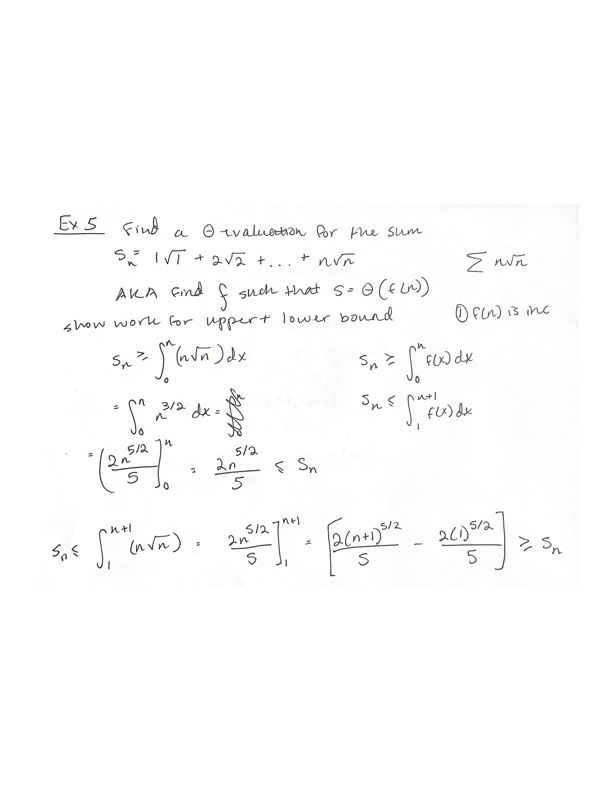
\includegraphics[scale=0.75]{ex5.png}

Lower bound:

$(2/5)n^{5/2} <= S$

\textcolor{red}{$S = \Theta(n^{5/2})$}

\bigskip Upper bound:

\smallskip$(2/5)(n+1)^{5/2} >= S$

$(n+1)^{5/2} >= S$

\smallskip\textcolor{red}{$S = \Theta((n+1)^{5/2})$}

\end{document}
